\section{Planning Approach Results}

\begin{figure}[t]
    \centering
    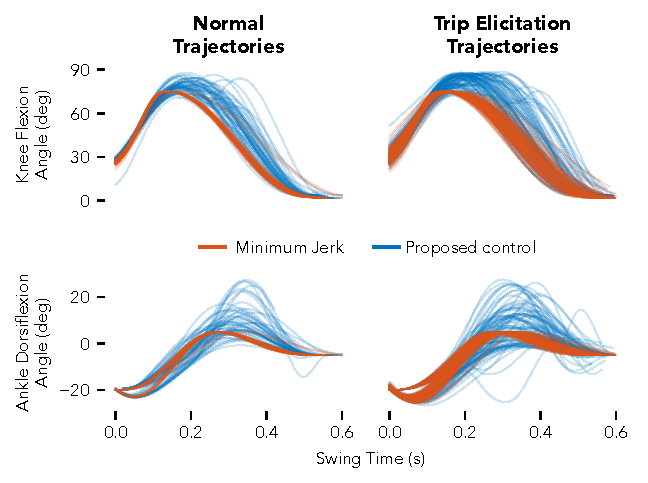
\includegraphics[width=\columnwidth]{trajectories_annotated}
    \caption{Knee and ankle trajectories produced during normal walking and
    while eliciting trips. To avoid tripping during trip elicitation trials,
    trajectories generated by the proposed approach often flex the knee to a
    greater degree and for longer before quickly extending at the end of swing.
    At the ankle joint we see overall greater variability in the generated
    trajectories during the trip elicitation condition versus normal walking.}
    \label{fig:trajectories}
\end{figure}

\Cref{fig:trajectories} shows the knee and ankle swing trajectories generated by
the proposed control (blue) and by a standard jerk minimization control (red)
during normal walking and trip elicitation. During undisturbed walking, the
trajectories produced by both control strategies are similar. However, the
proposed control strategy has a tendency to keep the knee flexed for longer and
then extends it faster towards the end of swing. In addition, in a few steps,
the proposed controller flexed the ankle significantly more than did the
standard minimum jerk control.  These trends are exaggerated during trip
elicitation. There are more knee trajectories in which the knee stays flexed for
longer, thereby creating more ground clearance. In addition, the ankle flexes
earlier, which will help to create more foot clearance when the hip is suddenly
lowered in early swing. 

We used video and audio recordings of the trials, as well as data from the
prosthesis, to manually classify trips as those swing trajectories that end with
toe strike or during which the foot scuffed on the ground. We find that over the
ten minutes of walking, the minimum jerk control produced 109 trips while the
proposed approach produced 35 trips, reducing the trip rate by 68\%.

\begin{figure}[t]
    \centering
    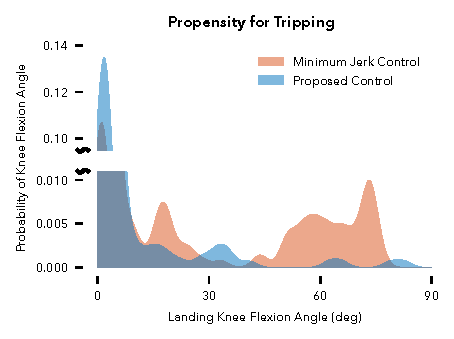
\includegraphics[width=\columnwidth]{prob_landing_angles}
    \caption{Kernel density estimate of the probability of various landing knee
    flexion angles with the proposed swing control (blue) and standard min-jerk
    swing control (red). Large landing knee angles indicate premature toe
    contact during swing.}
    \label{fig:p_landing_angle}
\end{figure}

To further examine the performance of the two control strategies, we used kernel
density estimates of the landing knee flexion angle, a measure of the propensity
for tripping, and integrated ground reaction force (GRF) during swing, a measure
of the propensity for foot scuffing. \Cref{fig:p_landing_angle} shows the
distributions of the landing angle of the prosthesis at the end of swing for the
proposed swing control (blue) and for the standard minimum jerk swing control
(red) during the trip elicitation condition. We observe the minimum jerk control
is much more likely to generate a swing trajectory that ends prematurely with a
large knee flexion angle, which is indicative of toe contact instead of heel
contact at the end of swing.  The distributions of the integrated GRFs suggests
the minimum jerk control produced a larger percentage of swings with high ground
reaction forces than the proposed control, indicating an increased frequency and
severity of toe scuffing during swing (\cref{fig:p_grf}). 
\begin{figure}[t]
    \centering
    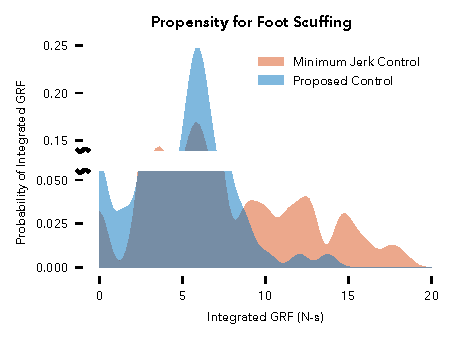
\includegraphics[width=\columnwidth]{prob_grf}
    \caption{Kernel density estimate of the probability of various integrated
    ground reaction force values for the proposed swing control (blue) and
    standard min-jerk swing control (red). Large integrated GRF during the swing
    phase is indicative of the toe scuffing on the ground.}
    \label{fig:p_grf}
\end{figure}

We can also ask the question, ``For steps during which the prosthesis used
trajectories generated by the proposed control, would the user have tripped had
the prosthesis used a minimum jerk trajectory?'' To answer this question, we can
use the kinematics model shown in \cref{fig:kinematics} along with ground truth
hip height and hip angle data captured via a motion capture system, to estimate
the location of the toe had the knee and ankle perfectly followed the desired
trajectories produced by each control scheme. This analysis predicts that the
prosthesis would have tripped or scuffed the toe on the ground during $22\%$ of
the steps if we had used the minimum jerk trajectory. In contrast, it predicts a
trip or scuff rate of $5\%$ had we perfectly followed the trajectories generated
by the proposed control.

\begin{figure}[t]
    \centering
    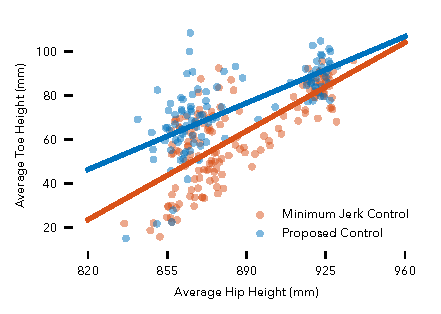
\includegraphics[width=\columnwidth]{toe_vs_hip_height}
    \caption{Average toe height vs average hip height for the proposed swing
    control (blue) and standard min-jerk swing control (red). The toe height
    during swing is less sensitive to the hip height when using the proposed
    swing control than when using the min-jerk swing control.}
    \label{fig:toe_vs_hip}
\end{figure}

Finally, \cref{fig:toe_vs_hip} shows the relationship between the average
toe and hip heights during swing for both control schemes. The toe height of the
prosthesis when controlled by the proposed control is less sensitive to
decreases in the hip height than it is when using the standard minimum jerk
control.
